The derivation of the Floquet Fermi golden rule for our quantum Hall system with the help of $t-t'$ formalism is given here in detail. The $t$-$t'$-Floquet states \cite{grifoni98,wackerl20}
\begin{equation} \label{eq_c1}
  \ket{\psi_{n,m}(t,t')} =
  \exp(-\frac{i}{\hbar}\varepsilon_{n} t)\ket{\phi_{n,m}(t')}.
\end{equation}
derived by seperating the aperiodic and periodic components of Eq.~(\ref{eq_12}), fullfill the $t$-$t'$-Schrödinger equation \cite{grifoni98,wackerl20}
\begin{equation} \label{eq_c2}
  i \hbar \pdv{t}\ket{\psi_{n,m}(t,t')} =
  H_F(t') \ket{\psi_{n,m}(t,t')},
\end{equation}
where \textit{Floquet Hamiltonian} defined as
\begin{equation} \label{eq_c3}
  H_F(t') \equiv
  H_e(t') - i\hbar \pdv{t'}.
\end{equation}
Next we can identify the the time evolution operator corresponding to the $t$-$t'$-Schrödinger equation
\begin{equation} \label{eq_c4}
  U_F(t,t_0;t') = \exp(-\frac{i}{\hbar}H_F(t')\qty[t-t_0]),
\end{equation}
and the advantage of $t$-$t'$ formalism lies on this time evolution operator which avoids any time odering operatos \cite{wackerl20}.

For our scenario, consider a time-independent total perturbation $V(\vb{r})$ which has been switched on at the reference time $t=t_0$, then the $t$-$t'$-Schrödinger equation becomes
\begin{equation} \label{eq_c5}
  i \hbar \pdv{t}\ket{\Psi_{n,m}(t,t')} =
  \qty[H_F(t') + V(\vb{r})]\ket{\Psi_{n,m}(t,t')},
\end{equation}
by introducing new wave function $\Psi_{n,m}$ for the system with the given total perturabation. If $t\leq t_0$, both solutions of the Schrödinger equations (Eq.~(\ref{eq_c2}) and Eq.~(\ref{eq_c5})) coincide
\begin{equation} \label{eq_c6}
  \ket{\psi_{n,m}(t,t')} =\ket{\Psi_{n,m}(t,t')} \quad
  \text{when} \quad
  t \leq t_0.
\end{equation}
Now move into the interaction picture representation \cite{bruus04,mahan00} of the $t$-$t'$-Floquet state
\begin{equation} \label{eq_c7}
  \ket{\Psi_{n,m}(t,t')}_I = U_0^{\dagger}(t,t_0;t')
  \ket{\Psi_{n,m}(t,t')},
\end{equation}
and due to time independency, the perturbation in the interaction picture has the same form as Schrödinger picture
\begin{equation} \label{eq_c8}
  V_I(\vb{r}) = U_0^{\dagger}(t,t_0;t')V(\vb{r})U_0(t,t_0;t') =
  V(\vb{r}).
\end{equation}
This leads to the $t$-$t'$-Schrödinger eqution in the interction picture
\begin{equation} \label{eq_c9}
  i \hbar \pdv{t}\ket{\Psi_{n,m}(t,t')}_I =
  V_I(\vb{r})\ket{\Psi_{n,m}(t,t')}_I,
\end{equation}
with the recursive solution \cite{bruus04,mahan00}
\begin{equation} \label{eq_c10}
  \begin{aligned}
  \ket{\Psi_{n,m}(t,t')}_I = &\ket{\Psi_{n,m}(t_0,t')}_I \\
  &+
  \frac{1}{i\hbar}
  \int_{t_0}^t dt_1 \;
  V_I(\vb{r}) \ket{\Psi_{n,m}(t_1,t')}_I.
  \end{aligned}
\end{equation}
Iterating the solution only upto the first order (Born approximation) we obtain
\begin{equation} \label{eq_c11}
  \begin{aligned}
    \ket{\Psi_{n,m}(t,t')}_I \approx &\ket{\psi_{n,m}(t_0,t')} \\
    &+
    \frac{1}{i\hbar}
    \int_{t_0}^t dt_1 \;
    V_I(\vb{r}) \ket{\psi_{n,m}(t_0,t')}.
  \end{aligned}
\end{equation}

In addition, since our Floquet states create a basis we can represent any solution using these Floquet states
\begin{equation} \label{eq_c12}
  \ket{\Psi_{\alpha}(t,t')} = \sum_{\beta} a_{\alpha,\beta}(t,t')
  \ket{\psi_{\beta}(t,t')}.
\end{equation}
where we used a single notation to represent two quantum numbers; $\alpha \equiv (n_{\alpha},m_{\alpha})$ and $\beta \equiv (n_{\beta},m_{\beta})$.
Then we can identify the \textit{scattering amplitude} as $a_{\alpha,\beta}(t,t') =
\braket{\psi_{\beta}(t,t')}{\Psi_{\alpha}(t,t')}$ and this can evaluate with
\begin{equation} \label{eq_c13}
  \begin{aligned}
  a_{\alpha,\beta}(t,t') = &
  \braket{\psi_{\beta}(t,t')}{\psi_{\alpha}(t,t')} \\
  &+
  \frac{1}{i\hbar}
  \int_{t_0}^t dt_1 \;
  \bra{\psi_{\beta}(t_1,t')}
  V(\vb{r}) \ket{\psi_{\alpha}(t_1,t')}.
  \end{aligned}
\end{equation}
Since the $t$-$t'$-Floquet states are orthonormal and assuming $t_0 = 0$ and $\alpha \neq \beta$ this leads to
\begin{equation} \label{eq_c14}
  a_{\alpha,\beta}(t,t') =
  -
  \frac{i}{\hbar}
  \int_{0}^t dt_1 \;
  \bra{\psi_{\beta}(t_1,t')}
  V(\vb{r}) \ket{\psi_{\alpha}(t_1,t')}.
\end{equation}

Now consider a scattering event from a $t$-$t'$-Floquet state $\ket{\psi_{\beta}(t,t')} $ into another $t$-$t'$-Floquet state $\ket{\Psi_{\alpha}(t,t')}$ with constant quansienergy $\varepsilon$:
\begin{equation} \label{eq_c15}
  \begin{aligned}
  \ket{\psi_{\beta}(t,t')} &= \exp(-\frac{i}{\hbar}\varepsilon_{\beta} t)
  \ket{\phi_{\beta}(t')} \\
  &
  \longrightarrow
  \ket{\Psi_{\alpha}(t,t')} = \exp(-\frac{i}{\hbar}\varepsilon t)
  \ket{\Phi_{\alpha}(t')}.
  \end{aligned}
\end{equation}
\begin{figure}[b]
  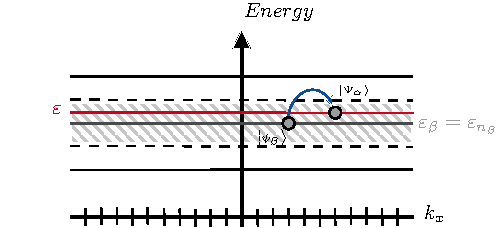
\includegraphics[scale=1.0]{figures/fig_2.pdf}
  \caption{Scattering from $\ket{\psi_{\beta}(t,t')}$ to constant energy state $\ket{\Psi_{\alpha}(t,t')}$ due to scattering potential created by impurities.}
  \label{fig_2}
\end{figure}
It is important to remember that a state of this considering system can be represented by two independent quantum numbers: $n$ represents the landau level and $m$ represents the qunatized momentum in $x$-direction. The scattering amplitutde for this scattering scenario can be calculated using the equation derived in Eq.~(\ref{eq_c14})
\begin{equation} \label{eq_c16}
  \begin{aligned}
    a_{\alpha\beta}(t,t') =
    -\frac{i}{\hbar}
    \int_{0}^t dt_1 \;
    e^{\frac{i}{\hbar}\qty(\varepsilon_{\beta} - \varepsilon)t_1}
    \bra{\phi_{\beta}(t')}
    V(\vb{r}) \ket{\phi_{\alpha}(t')},
  \end{aligned}
\end{equation}
and assuiming for a long time $t \rightarrow \infty$, we can turn this integral into a delta distrubution
\begin{equation} \label{eq_c17}
  \begin{aligned}
    a_{\alpha\beta}(t') =
    -2\pi i \delta(\varepsilon_{\beta} - \varepsilon)Q,
  \end{aligned}
\end{equation}
where $Q \equiv \bra{\phi_{\beta}(t')}
V(\vb{r}) \ket{\phi_{\alpha}(t')}$ and using completeness properties we can re-write this as
\begin{equation} \label{eq_c18}
    Q =
    \sum_{\vb{k}}\sum_{\vb{k'}}
    \braket{\phi_{\beta}(t')}{\vb{k'}}
    \mel{\vb{k'}}{V(\vb{r})}{\vb{k}}
    \braket{\vb{k}}{\phi_{\alpha}(t')},
\end{equation}
and seperating $x$ and $y$ directional momentums we can derive (we already assumed that $L_y \rightarrow \infty$)
\begin{equation} \label{eq_c19}
    Q =
    \sum_{k_x}\sum_{{k'}_x}
    \int_{-\infty}^{\infty} \int_{-\infty}^{\infty} dk_y d{k'}_y \;
    V_{\vb{k'},\vb{k}}
    \phi_{\beta}^{\dagger}(\vb{k'},t')
    \phi_{\alpha}(\vb{k},t').
\end{equation}
with $V_{\vb{k'},\vb{k}} \equiv \mel{\vb{k'}}{V(\vb{r})}{\vb{k}}$.

Since the perturbation potential $V(\vb{r})$ is assumed to be formed by an ensemble of randomly distributed impurities, consider $N_{imp}$ identical impurities positioned at randomly distributed but fixed positions $\vb{r}_i$. Then scattering potential $V(\vb{r})$ is given by the sum over uncorrelated single impurity potentials $\upsilon(\vb{r})$
\begin{equation} \label{eq_c20}
  V(\vb{r}) \equiv
  \sum_{i=1}^{N_{imp}}
  \upsilon (\vb{r}-\vb{r}_i).
\end{equation}
Next we model the perturbation $V(\vb{r})$ as a Gaussian random potential where one can choose the zero of enerrgy such that the potential is zero on average. This model is characterized by \cite{akkermans10}
\begin{subequations}
\begin{equation} \label{eq_c21a}
  \expval{\upsilon(\vb{r})}_{imp} =0,
\end{equation}
\begin{equation} \label{eq_c21b}
  \expval{\upsilon(\vb{r})\upsilon(\vb{r'})}_{imp} = \Upsilon(\vb{r}-\vb{r'}),
\end{equation}
\end{subequations}
where $\expval{\cdot}_{imp}$ denoted the average over realizations of the impurity disorder and $\Upsilon(\vb{r}-\vb{r'})$ is any decaying function depends only on $\vb{r}-\vb{r'}$. In addition, this model assume that $\upsilon (\vb{r}-\vb{r'})$ only dependes on the position difference $|\vb{r}-\vb{r'}|$ and it decays with a characteristic leangth $r_c$. Since this study considers the case where the waveleagth of radiation or scattering electrons is much faster than $r_c$, it is a good approximation to make two-point correlation function to be
\begin{equation} \label{eq_c22}
  \expval{\upsilon(\vb{r})\upsilon(\vb{r'})}_{imp} = \Upsilon_{imp}^2\delta(\vb{r}-\vb{r'}),
\end{equation}
where $\Upsilon_{imp}$ is stregth of the delta potential and a random potential $V(\vb{r})$ with this property is called white noise \cite{akkermans10}. Then we can model approximately the total scattering potential as
\begin{equation} \label{eq_c23}
  V(\vb{r}) =
  \sum_{i=1}^{N_{imp}}
  \Upsilon_{imp} \delta(\vb{r}-\vb{r}_i).
\end{equation}
Then we can calculate $V_{\vb{k'},\vb{k}}$ using this assumption as follows
\begin{subequations} \label{eq_c24}
\begin{align}
 V_{\vb{k'},\vb{k}} & =
 \mel**{\vb{k'}}{\sum_{i=1}^{N_{imp}}
 \Upsilon_{imp} \delta(\vb{r}-\vb{r}_i)}{\vb{k}} \label{eq_c24a} \\
 & =
 \sum_{i=1}^{N_{imp}}
 \int_{-\infty}^{\infty} dy\; \bigg[
 \frac{1}{\sqrt{L_xL_y}} e^{ik'_y y} \delta(y-y_i) \nonumber \\
 & \times \frac{1}{\sqrt{L_xL_y}} e^{-i{k}_y y}
 \mel**{k'_x}{\Upsilon_{imp} \delta(x-x_i)}{k_x} \bigg] \label{eq_c24b} \\
  & =
 \sum_{i=1}^{N_{imp}} \frac{1}{{L_xL_y}}
 e^{i(k'_y - k_y )y}
 \mel**{k'_x}{\Upsilon_{imp} \delta(x-x_i)}{k_x} \label{eq_c24c}.
\end{align}
\end{subequations}
Since $\upsilon (\vb{r})$ in momentum space is a constant value, each impurity  produce same impurity potential for every $x$-directional momentum pairs and assuming the total ncumber of scatterers $N_{imp}$ is macroscopically large, we can derive
\begin{subequations} \label{eq_c25}
  \begin{align}
    V_{\vb{k'},\vb{k}}
    & =
    V_{k'_x,k_x}
    \frac{N_{imp}}{L_y L_x} \int_{-\infty}^{\infty} dy_i\;
    e^{i\qty({k'}_y - k_y)y_i} \label{eq_c25a} \\
    & =
    \eta_{imp} V_{k'_x,k_x} \delta(k'_y - k_y), \label{eq_c25b}
  \end{align}
\end{subequations}
where
\begin{equation} \label{eq_c26}
  V_{{k'}_x,k_x} \equiv
  \mel**{k'_x}{\Upsilon_{imp} \delta(x-x_i)}{k_x}.
\end{equation}
is a constant value for every $i$ impurity and $\eta_{imp}$ is number of impurities in a unit area. It is important to notice that $\ket{k_x} = e^{-ik_xx}$.

Now using Eq.~(\ref{eq_9}) and Eq.~(\ref{eq_c25}) on Eq.~(\ref{eq_c19}), we obtain (with changing varable $t' \rightarrow t'$)
\begin{equation} \label{eq_c27}
  \begin{aligned}
    Q & =
    \sum_{k_x}\sum_{{k'}_x}
    {\eta_{imp} V_{{k'}_x,k_x}}
    \int_{-\infty}^{\infty} \int_{-\infty}^{\infty} dk_y d{k'}_y \;
    \delta({k'}_y - k_y)
    \\
    & \times
    \sqrt{L_x}
    \exp(
      i{k'}_y  \qty[d\sin(\omega t) + {y'}_0]
    )
    \tilde{\chi}_{n_{\beta}}\qty({k'}_y -b\cos(\omega t))
    \\
    & \times
    \sqrt{L_x}
    \exp(
      -ik_y  \qty[d\sin(\omega t) + y_0]
    )
    \tilde{\chi}_{n_{\alpha}}\qty(k_y -b\cos(\omega t)),
  \end{aligned}
\end{equation}
and this can simplify as
\begin{equation} \label{eq_c28}
  \begin{aligned}
    Q =
    \sum_{k_x}\sum_{{k'}_x}
    {\eta_{imp} L_x V_{{k'}_x,k_x}} I,
  \end{aligned}
\end{equation}
with
\begin{equation} \label{eq_c29}
  \begin{aligned}
    I \equiv
    \int_{-\infty}^{\infty} dk_y \;
    \tilde{\chi}_{n_{\beta}}\qty(k_y -b\cos(\omega t)) &
    \tilde{\chi}_{n_{\alpha}}\qty(k_y -b\cos(\omega t)) \\
    & \times
    \exp(
      -ik_y  \qty[y_0 - {y'}_0  ]
    ).
  \end{aligned}
\end{equation}
To avoid the energy exchange from external strong field and electrons, the applied radiation should be a purely dressing field. Therefore, the only effect of the dressing field on 2DEG is the renormalization of the probability of elastic electron scattering within the same Landau level $(n_{\alpha} = n_{\beta} =N)$. This transform the Eq.~(\ref{eq_c29}) to
\begin{equation} \label{eq_c30}
    I =
    \int_{-\infty}^{\infty} dk_y \;
    \tilde{\chi}_{N}^2 \qty(k_y -b\cos(\omega t))
    \exp(
      -ik_y  \qty[y_0 - {y'}_0  ]
    ).
\end{equation}
Using Fourier transform of Gauss-Hermite functions \cite{celeghini21} and convolution theorem \cite{arfken85,bracewell78} we can derive
\begin{equation} \label{eq_c31}
  \begin{aligned}
    I =
    {2\pi} &
    \exp(b[{y'}_0 - y_0]\cos(\omega t)) \\
    & \times
    \int_{-\infty}^{\infty} dy \;
    {\chi}_{N}\qty(y)
    {\chi}_{N}\qty(y_0 - {y'}_0 - y).
  \end{aligned}
\end{equation}
Therefore finally the scattering amplitude derived in Eq.~(\ref{eq_c17}) can be evaluated for given $k_x = 2\pi m_{\alpha}/L_x$ and $k'_x =  2\pi m_{\beta}/L_x$ as
\begin{equation} \label{eq_c32}
  \begin{aligned}
    a_{\alpha\beta}(k_x,k'_x,t)  =&
    -2\pi i
    \eta_{imp} L_x V_{{k'}_x,k_x}
    \delta(\varepsilon_{N} - \varepsilon)\\
    & \times
    \exp(b[{y'}_0 - y_0]\cos(\omega t))\\
    & \times
    \int_{-\infty}^{\infty} dy \;
    {\chi}_{N}\qty(y)
    {\chi}_{N}\qty(y_0 - {y'}_0 - y),
  \end{aligned}
\end{equation}
Since this scattering amplitude is time-periodic we can write this as a Fourier series expansion
\begin{equation} \label{eq_c33}
    a_{\alpha\beta}(k_x,k'_x,t) =
    \sum_{l=-\infty}^{\infty} a^l_{\alpha\beta}(k_x,k'_x) e^{-il\omega t}.
\end{equation}
In addition, using Jacobi-Anger expansion \cite{cuyt08,abramowitz64}
\begin{equation} \label{eq_c34}
    e^{iz\cos(\theta)} = \sum_{l=-\infty}^{\infty} i^l J_l\qty(z) e^{-il\theta},
\end{equation}
where $J_l(z)$ are Bessel functions of the first kind with $l$-th integer order and we can re-write the Eq.~(\ref{eq_c32}) as folllows
\begin{equation} \label{eq_c35}
  \begin{aligned}
    a_{\alpha\beta}(k_x,k'_x,t)  = &
    \sum_{l=-\infty}^{\infty}
    -2\pi i^{l+1}
    \eta_{imp} L_x V_{{k'}_x,k_x}
    \delta(\varepsilon_{N} - \varepsilon)\\
    & \times
    J_l\qty(b[{y'}_0 - y_0]) \\
    & \times
    \int_{-\infty}^{\infty} dy \;
    {\chi}_{N}\qty(y)
    {\chi}_{N}\qty(y_0 - {y'}_0 - y) e^{-il\omega t},
  \end{aligned}
\end{equation}
and then the Fourier series component can be identified as
\begin{equation} \label{eq_c36}
  \begin{aligned}
    a^l_{\alpha\beta}(k_x,k'_x) = &
    -2\pi i^{l+1}
    \eta_{imp} L_x V_{{k'}_x,k_x}\\
    & \times
    \delta(\varepsilon_{N} - \varepsilon)
    J_l\qty(b[{y'}_0 - y_0])\\
    & \times
    \int_{-\infty}^{\infty} dy \;
    {\chi}_{n_{\beta}}\qty(y)
    {\chi}_{n_{\beta}}\qty(y_0 - {y'}_0 - y).
  \end{aligned}
\end{equation}
Now define \textit{transition probability matrix}
\begin{equation} \label{eq_c37}
    \qty(A_{\alpha\beta})_{l,l'} \equiv
    a^l_{\alpha\beta}\qty[a^{l'}_{\alpha\beta}]^{*},
\end{equation}
and this becomes
\begin{equation} \label{eq_c38}
  \begin{aligned}
      \qty(A_{\alpha\beta})_{l,l'}(k_x,k'_x) = &
      \qty[{ 2 \pi \eta_{imp} L_x |V_{{k'}_x,k_x}|}]^2
      \delta^2(\varepsilon_{N} - \varepsilon) \\
      & \times
      J_l\qty(b[{y'}_0 - y_0]) J_{l'}\qty(g[{y'}_0 - y_0])\\
      & \times
      \qty|
      \int_{-\infty}^{\infty} dy \;
      {\chi}_{n_{\beta}}\qty(y)
      {\chi}_{n_{\beta}}\qty(y_0 - {y'}_0 - y)|^2.
  \end{aligned}
\end{equation}
Then desribing the square of the delta distribution using following procedure \cite{dini16,kibis14}
\begin{equation} \label{eq_c39}
    \delta^2(\varepsilon) =
    \delta(\varepsilon)\delta(0) =
    \frac{\delta(\varepsilon)}{2\pi \hbar}
    \int_{-t/2}^{t/2} e^{i0\times t'/\hbar} dt'\; =
    \frac{\delta(\varepsilon)t}{2\pi \hbar},
\end{equation}
and performing the time derivation of each matrix element yeild the \textit{transition amplitude matrix}:
\begin{equation} \label{eq_40}
  \begin{aligned}
    \Gamma_{\alpha\beta}^{ll'}(k_x,k'_x) = &
    \frac { 2\pi \eta_{imp}^2 L_x^2}{ \hbar} |V_{{k'}_x,k_x}|^2
    \delta(\varepsilon_{\beta} - \varepsilon)\\
    & \times
    J_l\qty(b[{y'}_0 - y_0]) J_{l'}\qty(g[{y'}_0 - y_0]) \\
    & \times
    \qty|
    \int_{-\infty}^{\infty} dy \;
    {\chi}_{N}\qty(y)
    {\chi}_{N}\qty(y_0 - {y'}_0 - y)|^2.
  \end{aligned}
\end{equation}

An impurity average of white noise potential allows to identify $\expval{|V_{{k'}_x,k_x}|^2} = V_{imp}$ and the inverse scattering time matrix is the sum over all momentum over the transition probability matrix
\begin{equation} \label{eq_41}
    \qty(\frac{1}{\tau(\varepsilon,k_x)})^{ll'}_{\alpha\beta} \equiv
    \frac{1}{L_x} \sum_{{k'}_x}
    \expval**{\Gamma_{\alpha\beta}^{ll'}({k'}_x,k_x)}_{imp},
\end{equation}
and applying the 1-dimentional momentum continuum limit $\sum_{{k'}_x} \longrightarrow {L_x}/{2\pi}\int d {k'}_x$ and this leads to
\begin{equation} \label{eq_42}
  \begin{aligned}
    \bigg(&\frac{1}{\tau(\varepsilon,k_x)}\bigg)^{ll'}_{\alpha\beta} \\
    & =
    \frac { 2\pi \eta_{imp}^2 L_x^2}{ \hbar}
    \frac{V_{imp}}{2\pi}
    \delta(\varepsilon_{\beta} - \varepsilon)\\
    & =
    \int_{-\infty}^{\infty} d {k'}_x
    J_l\qty(\frac{b\hbar}{eB}[{k}_x - {k'}_x])
    J_{l'}\qty(\frac{b\hbar}{eB}[{k}_x - {k'}_x]) \\
    & \times
    \qty|
    \int_{-\infty}^{\infty} dy \;
    {\chi}_{n_{\beta}}\qty(y)
    {\chi}_{n_{\beta}}\qty(\frac{\hbar}{eB} \qty[{k'}_x - {k}_x] - y)|^2.
  \end{aligned}
\end{equation}
Using subtitution $k'_x = k_1$ and $y = {\hbar{k_2}}/{eB}$ finally we can derive our expression for the inverse scattering time matrix for $N$-th Landau
level
\begin{equation} \label{eq_43}
  \begin{aligned}
    \bigg(&\frac{1}{\tau(\varepsilon,k_x)}\bigg)^{ll'}_{N} \\
    & =
    \frac { \eta_{imp}^2 L_x^2 \hbar V_{imp}}{\qty(eB)^2}
    \delta(\varepsilon - \varepsilon_{N})\\
    & \times
    \int_{-\infty}^{\infty} d k_1
    J_l\qty(\frac{b\hbar}{eB}[{k}_x - k_1])
    J_{l'}\qty(\frac{b\hbar}{eB}[{k}_x - k_1]) \\
    & \times
    \qty|
    \int_{-\infty}^{\infty} dk_2 \;
    {\chi}_{N}\qty(\frac{\hbar}{eB}k_2)
    {\chi}_{N}\qty(\frac{\hbar}{eB} \qty[k_1 - {k}_x - k_2])|^2.
  \end{aligned}
\end{equation}
